\chapter{Related work}\label{ch:related-work}
    In the following chapter provides an overview of research and state-of-the-art in the domain of modelling and simulation of traffic systems.
    Section~\ref{sec:foundational-studies} examines foundational studies that have shaped current understanding of modelling traffic systems, focusing on the methodologies and findings that are most relevant to this thesis.
    Section~\ref{sec:studies-closely-related-to-an-integrated-simulation-environment} focuses on studies that are more closely related to the proposed simulation environment and the challenges that had to be solved in order to create one such integration.
    Finally, Section~\ref{sec:summary-of-findings} summarises the findings of the literature review and identifies the used solutions for upcoming challenges encountered along the way of developing the integrated Simulation environment.
    By mapping out the state of the art, this chapter establishes the context for the subsequent discussion of the proposed approach and methodology in Chapter~\ref{ch:methods}.


    \section{Foundational studies}\label{sec:foundational-studies}
        The field of traffic science is divisible into multiple different sub-categories by the time span of the observed events.
        As described by Treiber et al. \cite{treiber2013traffic} there are Vehicle dynamics, Traffic flow dynamics and Transportation planning as the three major topics(see Table~\ref{tab:dilimination-of-traffic-flow-dynamics}).
        These fields are divisible even further as stated in table~\ref{tab:dilimination-of-traffic-flow-dynamics}.
        The proposed simulation environment would fall into the category of traffic flow dynamics using microscopic car following models.
        According to Treiber et al. this kind of simulation environments are best used to model reaction times, time gaps and the acceleration/breaking behaviors of vehicles in a traffic scenario.
        Driving behavior of vehicles in traffic flow dynamics are usually described by vehicle following (VF) models, which will be discussed further in the following sections.

        \begin{table}[ht]
            \centering
            \begin{tabular}{p{.1\linewidth} p{.2\linewidth} p{.2\linewidth} p{.4\linewidth}}
                \hline
                Time scale & Field & Models & Aspects of traffic (examples) \\ \hline \hline
                $\le 0.1 s$ & Vehicle dynamics & Sub-microscopic & Control of engine and breaks \\ \hline
                1 s & \multirow{4}{\linewidth}{Traffic flow dynamics}&\multirow{2}{\linewidth}{Car-following modells} & Reaction time, time gap \\
                10 s & & & Acceleration and deceleration \\\\
                1 min& & \multirow{2}{\linewidth}{Macroscopic models} & Cycle period of traffic lights \\
                10 min & & & Stop-and-go waves \\ \hline
                1 h & \multirow{5}{\linewidth}{Transportation planning} & \multirow{3}{\linewidth}{Route assignment traffic demand} & Peak hour \\
                1 day & & & Daily demand pattern \\
                1 year & & & Building/changing infrastructure \\\\
                5 years & &  \multirow{2}{\linewidth}{Statistics age pyramid} & Socioeconomic structure \\
                50 years & & & Demographic change \\ \hline

            \end{tabular}
            \caption{Delimitation of traffic flow dynamics from vehicular dynamics and transportation planning\cite{treiber2013traffic}}
            \label{tab:dilimination-of-traffic-flow-dynamics}
        \end{table}

        \subsection{Gazis-Herman-Rothery model}\label{subsec:gazis-herman-rothery-model}
            Vehicle following models have been researched for more than 70 years~\cite{pipes1953operational} and many such models have been developed since.
            One of the first widely known VF models is the Gazis-Herman-Rothery (GHR) model (see Eq \ref{eq:GHR}), which described the acceleration of a vehicle $n$ in a driving scenario with respect to the difference in speed $\Delta v$ to the leading vehicle $n-1$ and the distance to the leading vehicle $\Delta x$, at a point earlier in time, with $T$ being the reaction time of the driver\cite{Brackstone1999}.
            \begin{equation}
                a_n(t) = c v_n^m(t) \frac{\Delta v (t-T)}{\Delta x^{-1} (t-T)} \label{eq:GHR}
            \end{equation}

        \subsection{Gipps' model}\label{subsec:gipps-model}
            Gipps states in the paper proposing his own VF model (Gipps´ model), that most VF models up until then (1981) have generally been in the form of EQ~\ref{eq:general-form-vf-model-1981}, where $\tau = T$.
            One example for this general form is the GHR model, some more of those models are found in publications dating back to that time: \cite{newell1961nonlinear, lee1966generalization, bender1970flow}.
            \begin{equation}
                a_n(t+\tau) = l_n \frac{[v_{n-1} - v_n]^k}{[x_{n-1} - x_n]^m}\label{eq:general-form-vf-model-1981}
            \end{equation}
            As pointed out by Philip A. Seddon, the fact, that the time interval between subsequent calculations was given by the reaction time was an undesired characteristic of these models\cite{seddon1972program}, which could be overcome by storing a considerable amount of historical data, which was undesired at the time.
            The second pain point of these models, by today's standards maybe the more relevant point, was the existence of parameters $l_n$,$k$,$m$ (EQ~\ref{eq:general-form-vf-model-1981}), that have no identifiable connection to driver or vehicle characteristics\cite{gipps1981behavioural}.

            To address these deficits, Gipps proposed a new vehicle following model describing the speed of a vehicle at a point in time, in contrast to describing the acceleration of a vehicle at a point in time.
            The following form of the Gipps` model is not the form of the original publication, but the form from~\cite{treiber2013traffic}, which introduces a save speed $v_{save}$ for simplification.
            As stated by Treiber et al. the model is conseptually unchanged.
            The GHR model calculates the speed of a vehicle with respect to the desired acceleration $a$, deceleration $b$, Desired speed $v_0$ and minimum distance $s_0$.
            \begin{align}
                v_{save} (s, v_l) &= -b*\Delta t + \sqrt{b^2 \Delta t^2 - v_l^2 + 2b (s-s_0)} \\
                v(t+ \Delta t) &= min[v+a\Delta t, v_0, v_{save}(s,v_l)] \label{eq:gipps-model-simplified}
            \end{align}
            With the concept of the save speed depending on the distance to the front vehicle $s$ and its speed $v_l$, the gipps` model assembles one of the simplest complete %TODO: explain model completeness
            and accident-free models possible.
            The accident-free characteristic of the model is guaranteed with the assumptions that deceleration and reaction times are constant~\cite{treiber2013traffic}.
            In essence the gipps` model chooses the minimum between the desired speed, the safe speed or the speed that max acceleration would result in the next time step.
            Problem with this model is, that as stated by Treiber et al. it produces an unrealistic acceleration profile.

        \subsection{Intelligent driver model}\label{subsec:intelligent-driver-model}
            The time-continuous Intelligent driver model produces a realistic acceleration profile, since one of the requirements for forming the IDM is that the acceleration function $\dot{v}(s,v,v_l)$ is continuously differentiable in every three variables and thus producing smooth transitions between eg. breaking and acceleration phases.
            Another design criteria of the IDM is that the equilibrium distance\footnotemark has to be larger than the "safe" distance ($v*T + v_0$), with $v$ being the current speed, $T$ being the desired distance between vehicles in seconds and $v_0$ representing the "bumper-to-bumper" distance (min distance kept between vehicles), which ensures the accident-free characteristic of that model.
            \footnotetext{The Distance, that is required between vehicles to stay in a steady-state equilibrium, which means, in a homogenous convoy the distance between all vehicles and the speed is the same. Furthermore the acceleration has to be 0 for every vehicle to be in a steady-state eqilibrium. \cite{treiber2013traffic, treiber2000IDM} }

            \begin{align}
                s^*(v,\Delta v) = s_0 + \max\left( 0, vT + \frac{v \Delta v}{2 \sqrt{ab}} \right) \label{eq:IDM-s-star} \\
                \dot{v}(s,v,v_l) = a * \left[ 1- \left(\frac{v}{v_0}\right)^\delta  - \left( \frac{s^*(v, \Delta v)}{s} \right)^2\right] \label{eq:IDM}
            \end{align}

            The IDM (see EQ~\ref{eq:IDM})is constructed from 2 pieces, the first part is comparing the current speed to the desired speed: $\left(\frac{v}{v_0}\right)^\delta$.
            The second part is comparing the current distance to the desired distance $s^*$ (see EQ~\ref{eq:IDM-s-star}): $\left( \frac{s^*(v, \Delta v)}{s} \right)^2$ \cite{treiber2013traffic, treiber2000IDM}.

            The advantage of using an intuitive model like gipps` model or the IDM, is that they are easy to configure by some simple understandable parameters (including vehicle and driver specific numbers).
            For example the configuration of the IDM consists of six parameters controlling the behavior of vehicles, with default values used by TraffSim (see Table~\ref{tab:IDM-Default-Values})~\cite{treiber2013traffic,backfrieder2013traffsim,backfrieder2014traffsim}.
            The Implementation in TraffSim includes two additional parameters, determining the maximum possible acceleration $a_{max}$ and deceleration $b_{max}$, which act as a hard limit for the acceleration function.
            The value of $b_{max}$ for example models the physical limit of the breaks of a car.
            \begin{table}
                \centering
                \begin{tabular}{l c c}
                    Parameter & TraffSim default Value & Acceptable Range \\
                    \hline
                    Comfortable acceleration $a$ & $2 \si{\m\per\s\squared}$ & $ 0 < a < a_{max}$\\
                    Comfortable deceleration $b$ & $-2 \si{\m\per\s\squared}$ & $ b_{max} < b < 0$\\
                    Desired Speed $v_0$ & $25 \si{\m\per\s}$ & $v_0 > 0$ \\
                    Minimum bumper-to-bumper distance $s_0$ & $2 \si{\m}$ & $s_0 > 0$ \\
                    Time gap $T$ & $1.5 \si{\s}$ & $T > 0$\\
                    Acceleration exponent $\delta$ \footnotemark& 4 & $\delta >  0$\\
                \end{tabular}
                \caption{Default Values for IDM}
                \label{tab:IDM-Default-Values}
            \end{table}
            \footnotetext{Dimensionless factor determining the rate at wich the vehicle`s acceleration decreases as it approaches its desired velocity}

        \subsection{Micro traffic simulation}\label{subsec:micro-traffic-simulation}
            The aforementioned vehicle following models are among others, implemented in a traffic simulator.
            Since one such simulator is a key building block of the desired simulation environment, the next section focuses on the micro traffic simulation environments available in literature.
            Special focus will be placed onto the micro traffic simulator TraffSim~\cite{backfrieder2013traffsim,backfrieder2014traffsim}, developed in house at Hagenberg.

            The first notable example is MovSim~\cite{Treiber2010}, which is an open source, free to use traffic simulator developed by a team at TU Dresden.
            MovSim implements the IDM (see Section~\ref{subsec:intelligent-driver-model}) among other vehicle following model which is responsable for the longitudinal movement of vehicles.
            For transversal movement of vehicles, MovSim utilizes the MOBIL model~\cite{kesting2007general}, which is a model for lane changing working alongside a variety of VF models.
            MovSim is primary source for sample implementations of VF models described by Treiber et al. (in~\cite{treiber2013traffic}).
            A picture of the web based user interface is depicted in Figure~\ref{fig:mov-sim-ui}.

            \begin{figure}
                \centering
                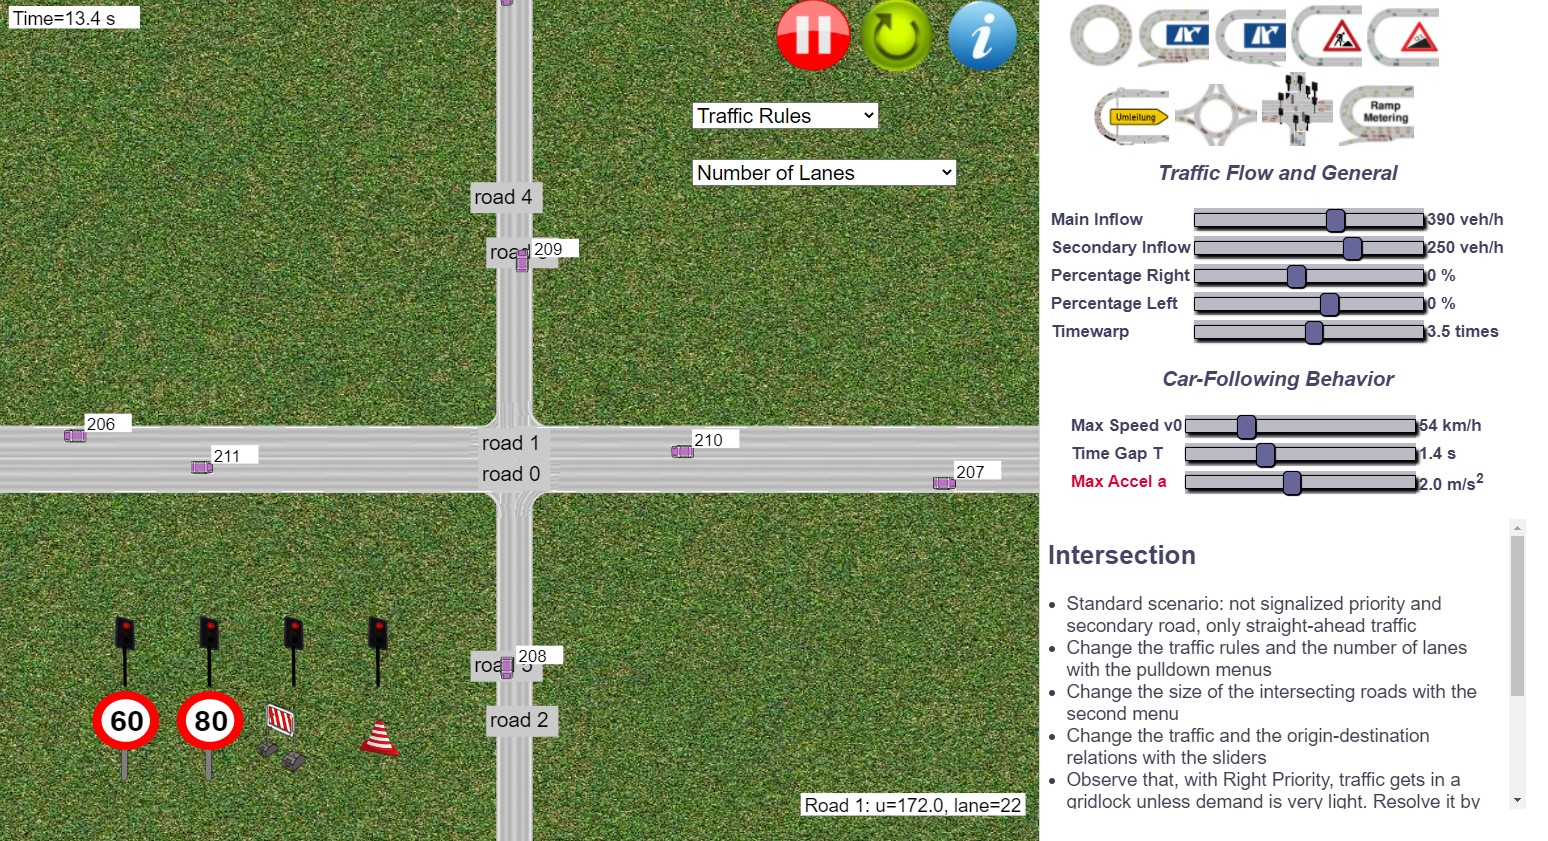
\includegraphics[width=0.7\textwidth]{Movsim}
                \caption{MovSim user interface~\cite{MovSimUI}}
                \label{fig:mov-sim-ui}
            \end{figure}

            One of the most popular traffic simulation environments is Eclipse SUMO~\cite{Behrisch2011SUMOS}, which is


    \section{Studies closely related to an integrated simulation environment}\label{sec:studies-closely-related-to-an-integrated-simulation-environment}

    \section{Summary of findings}\label{sec:summary-of-findings}

    As described by Treiber et al., both of these simulators are located in the field of traffic flow dynamics.



    \section{Microscopic traffic simulation}\label{sec:microscopic-traffic-simulation}


    \section{Driving simulation}\label{sec:driving-simulation}


